\documentclass[a4paper, 11pt, oneside]{article} % A4 paper size, default 11pt font size and oneside for equal margins

\newcommand{\plogo}{\fbox{$\mathcal{PL}$}} % Generic dummy publisher logo

\usepackage[utf8]{inputenc} % Required for inputting international characters
\usepackage[T1]{fontenc} % Output font encoding for international characters
\usepackage{fouriernc} % Use the New Century Schoolbook font
\usepackage{amsmath}
\usepackage{graphicx}
\usepackage{subcaption}
\usepackage{enumitem}
\usepackage{multicol}
\usepackage{tikz}
\usepackage{mathtools}
\usepackage{hyperref}
\usepackage{listings}

\DeclarePairedDelimiter\ceil{\lceil}{\rceil}
\DeclarePairedDelimiter\floor{\lfloor}{\rfloor}


%----------------------------------------------------------------------------------------
%	TITLE PAGE
%----------------------------------------------------------------------------------------

\begin{document} 

\begin{titlepage} % Suppresses headers and footers on the title page

	\centering % Centre everything on the title page
	
	\scshape % Use small caps for all text on the title page
	
    \vspace*{\baselineskip} % White space at the top of the page
    
    \begin{figure}

        \centering

        
\includegraphics[width=0.7\textwidth]{image/logo}

    \end{figure}
	
	%------------------------------------------------
	%	Title
	%------------------------------------------------
	
	\rule{\textwidth}{1.6pt}\vspace*{-\baselineskip}\vspace*{2pt} % Thick horizontal rule
	\rule{\textwidth}{0.4pt} % Thin horizontal rule
	
	\vspace{0.75\baselineskip} % Whitespace above the title
	
	{\LARGE Data Compression} % Title
	
	\vspace{0.75\baselineskip} % Whitespace below the title
	
	\rule{\textwidth}{0.4pt}\vspace*{-\baselineskip}\vspace{3.2pt} % Thin horizontal rule
	\rule{\textwidth}{1.6pt} % Thick horizontal rule
	
	\vspace{2\baselineskip} % Whitespace after the title block
	
	%------------------------------------------------
	%	Subtitle
	%------------------------------------------------
	
	Homework 1 % Subtitle or further description
	
	\vspace*{3\baselineskip} % Whitespace under the subtitle
	
	%------------------------------------------------
	%	Editor(s)
	%------------------------------------------------
	
	Student ID:

	\vspace{0.5\baselineskip}

	{\scshape 108368017}

	\vspace{0.5\baselineskip}

	Student: 
	
	\vspace{0.5\baselineskip} % Whitespace before the editors

	% {\scshape 108368017 \hspace{10mm}}
	{\scshape\Large Zi-Yang Lin } % Editor list

	\vspace{0.5\baselineskip} % Whitespace before the editors


	Advisor:

	\vspace{0.5\baselineskip} % Whitespace before the editors
	
	{\scshape\Large Chiu-Ching Tuan} % Editor list
	
	\vspace{0.5\baselineskip} % Whitespace below the editor list
	
	\textit{National Taipei University of Technology} % Editor affiliation
	
	\vfill % Whitespace between editor names and publisher logo
	
	%------------------------------------------------
	%	Publisher
	%------------------------------------------------
	
	% \plogo % Publisher logo
	
	\vspace{0.3\baselineskip} % Whitespace under the publisher logo
	
	2019 % Publication year
	
	% {\large publisher} % Publisher

\end{titlepage}

%----------------------------------------------------------------------------------------
\clearpage

\section*{Problem 1}
Let X be a random variable with an alphabet $H=\{1, 2, 3, 4, 5\}$. Please determine 
$H(X)$ for the following three cases of probability mass function $p(i)=prob[X=i]$.~(15\%)

\begin{enumerate}[label=(\alph*)]
	\item $p(1)=p(2)=\frac{1}{2}$
	\subsection*{Ans:}
	\begin{align*}
		H(X)&=-(\frac{1}{2})\log_{2}(\frac{1}{2})+\frac{1}{2}\log_{2}(\frac{1}{2})) \\
			&=-(-\frac{1}{2}-\frac{1}{2})  \\
			&= 1 ~bits/symbol
	\end{align*}
	\label{p:1-a}
	\item $p(i)=\frac{1}{4}, for~i = 1, 2, 3, ~and~p(4) = p(5) = \frac{1}{8}$
	\subsection*{Ans:}
	\begin{align*}
		H(X)&=-(3\times \frac{1}{4}\log_{2}(\frac{1}{4})+2\times 
				\frac{1}{4}\log_{2}(\frac{1}{4})) \\
			&=-(-1.5-0.75)  \\
			&= 2.25 ~bits/symbol
	\end{align*}
	\label{p:1-b}
	\item $P(i)=2^{-i}, for~i = 1, 2, 3, 4,and~p(5) =  \frac{1}{16}$
	\subsection*{Ans:}
	\begin{align*}
		H(X)&=-(\sum_{i=1}^{4} 2^{-i}\log_{2}2^{-i}+\frac{1}{16}\log_{2}\frac{1}{16}) \\
			&=-(0.5\times(-1)+0.25\times(-2)+0.125\times(-3)+0.0625\times(-4)
			  +0.0625\times(-4)) \\
			&= 1.875 ~bits/symbol
	\end{align*}
	\label{p:1-c}
	
\end{enumerate}

\clearpage

\section*{Problem 2}
Design a Huffman code C for the source in Problem 1.

\begin{enumerate}[label=(\alph*)]
	\item Specify your codewords for individual pmf model in Problem 1.
	\subsection*{Ans:}
	\textbf{\ref{p:1-a}}
	\begin{multicols}{2}
		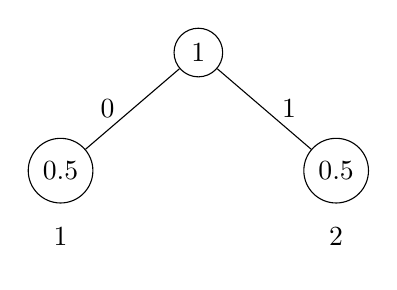
\begin{tikzpicture}[level distance=1.5cm,
							level 1/.style={sibling distance=3.5cm},
							level 2/.style={sibling distance=1cm}]
			\tikzstyle{every node}=[circle, draw]
			\node (Root) {1}
				child {
					node  (a1)  {$0.5$} 
					edge from parent node[left,draw=none] {0}
				}
				child {
					node  (a2) {$0.5$}
					edge from parent node[right,draw=none] {1}
				};

			\begin{scope}[nodes = {below = 15pt, draw = none}]
				\node at (a1) {$1$};
				\node at (a2) {$2$};
			\end{scope}

		\end{tikzpicture} 

		\columnbreak
	
		\null \vfill
		\begin{tabular}{ |c|c|c| } 
			\hline
			Alphabet & P  & Codeword \\
			\hline
			1 & 0.5 & 0 \\ 
			2 & 0.5 & 1 \\  
			\hline
			\end{tabular}
		\null \vfill
	\end{multicols}

	\vspace{5em}

	\subsection*{\ref{p:1-b}}
  	\begin{multicols}{2}
		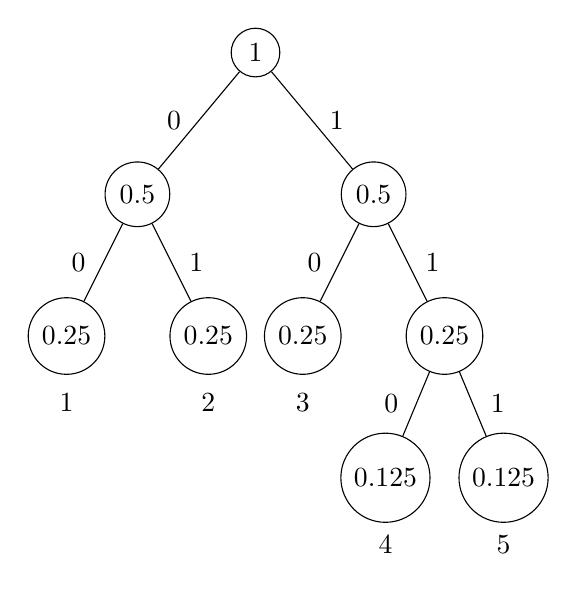
\begin{tikzpicture}[level distance=1.8cm,
			level 1/.style={sibling distance=3.0cm},
			level 2/.style={sibling distance=1.8cm},
			level 3/.style={sibling distance=1.5cm}]
		\tikzstyle{every node}=[circle, draw]
			\node (Root) {1}
				child {
					node {$0.5$} 
					child { node (a1) {$0.25$}
							edge from parent node[left,draw=none] {0}
					}
					child { node (a2) {$0.25$}
							edge from parent node[right,draw=none] {1}
					}
					edge from parent node[left,draw=none] {0}
				}
				child {
					node {$0.5$}
					child { node (a3) {$0.25$}
							edge from parent node[left,draw=none] {0}
					}
					child { node {$0.25$}
							child { node (a4) {$0.125$}
									edge from parent node[left,draw=none] {0}
							}
							child { node (a5) {$0.125$}
									edge from parent node[right,draw=none] {1}
							} 
						edge from parent node[right,draw=none] {1}
					}
					edge from parent node[right,draw=none] {1}
				};

				\begin{scope}[nodes = {below = 15pt, draw = none}]
					\node at (a1) {$1$};
					\node at (a2) {$2$};
					\node at (a3) {$3$};
					\node at (a4) {$4$};
					\node at (a5) {$5$};
				\end{scope}

		\end{tikzpicture} 
		
		\columnbreak
			
		\vfill
		\begin{tabular}{ |c|c|c| } 
			\hline
			Alphabet & P & Codeword \\
			\hline
			1 & 0.25  & 00  \\ 
			2 & 0.25  & 01  \\
			3 & 0.25  & 10  \\
			4 & 0.125 & 110 \\
			5 & 0.125 & 111 \\
			\hline
		\end{tabular}
		\vfill
	\end{multicols}
	  
	\clearpage

	\textbf{\ref{p:1-c}}
  	\begin{multicols}{2}
		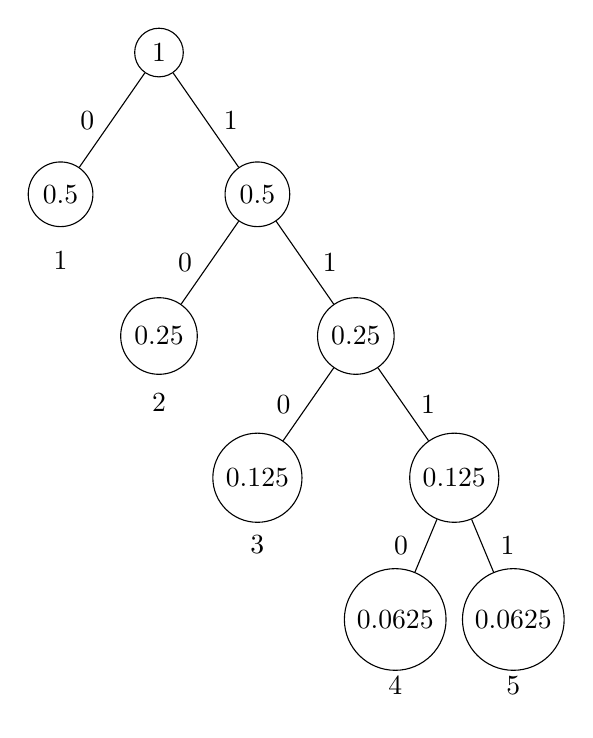
\begin{tikzpicture}[level distance=1.8cm,
			level 1/.style={sibling distance=2.5cm},
			level 2/.style={sibling distance=2.5cm},
			level 3/.style={sibling distance=2.5cm},
			level 4/.style={sibling distance=1.5cm}]
			\tikzstyle{every node}=[circle,draw]
		\node (Root) {1}
			child {
				node (a1) {$0.5$} 
				edge from parent node[left,draw=none] {0}
			}
			child {
				node {$0.5$}
				child { node (a2) {$0.25$} 
					edge from parent node[left,draw=none] {0}
				}
				child { node {$0.25$}
					child { node (a3) {$0.125$}
						edge from parent node[left,draw=none] {0}
					}
					child { node {$0.125$}
						child { node (a4) {$0.0625$}
							edge from parent node[left,draw=none] {0}
						}
						child { node (a5) {$0.0625$}
						edge from parent node[right,draw=none] {1}
						}
						edge from parent node[right,draw=none] {1}
					}
					edge from parent node[right,draw=none] {1}
				}
				edge from parent node[right,draw=none] {1}
			};

			\begin{scope}[nodes = {below = 15pt, draw = none}]
				\node at (a1) {$1$};
				\node at (a2) {$2$};
				\node at (a3) {$3$};
				\node at (a4) {$4$};
				\node at (a5) {$5$};
			\end{scope}

	  	\end{tikzpicture}
	  
      	\columnbreak

    	\vfill
      	\begin{tabular}{ |c|c|c| } 
        	\hline
        	Alphabet & P  & Codeword \\
        	\hline
        	1 & 0.5     & 0 \\ 
        	2 & 0.25    & 10 \\  
        	3 & 0.125   & 110 \\  
        	4 & 0.0625  & 1110 \\  
        	5 & 0.0625  & 1111 \\  
        	\hline
        \end{tabular}
		\vfill
	\end{multicols}

	\vspace{2em}

	\item Compute the expected codeword length and compare with the entropy for your 
	codes in (a).
	\subsection*{Ans:}
	\textbf{\ref{p:1-a}}
  	\begin{align*}
    	expected~codeword~length&=0.5 \times 1 + 0.5 \times 1 \\
                            &=1 ~bits/symbol~\textbf{(Equal Entropy)}
  	\end{align*}
  	\textbf{\ref{p:1-b}}
  	\begin{align*}
    	expected~codeword~length&=0.25 \times 2 + 0.25 \times 2 + 0.25 \times 2 + 
                              0.125 \times 3 + 0.125 \times 3 \\
                            &=2.25 ~bits/symbol~\textbf{(Equal Entropy)}
  	\end{align*}
  	\textbf{\ref{p:1-c}}
  	\begin{align*}
    	expected~codeword~length&=0.5 \times 1 + 0.25 \times 2 + 0.125 \times 3 + 
                              0.0626 \times 4 + 0.0625 \times 4 \\
                            &=4.125 ~bits/symbol~\textbf{(NOT Equal Entropy)}
	\end{align*}
	  
	\clearpage

	\item Design a code with minimum codeword length variance for the pmf model in Problem 1.(b)
	\subsection*{Ans:}
	\begin{multicols}{2}
		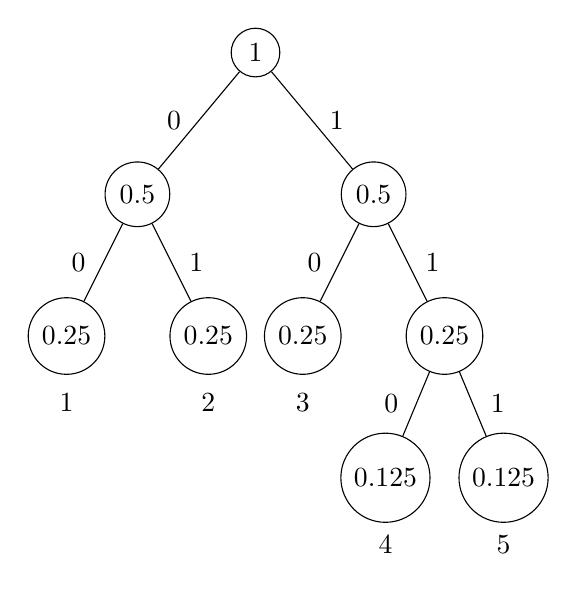
\begin{tikzpicture}[level distance=1.8cm,
			level 1/.style={sibling distance=3.0cm},
			level 2/.style={sibling distance=1.8cm},
			level 3/.style={sibling distance=1.5cm}]
		\tikzstyle{every node}=[circle, draw]
			\node (Root) {1}
				child {
					node {$0.5$} 
					child { node (a1) {$0.25$}
							edge from parent node[left,draw=none] {0}
					}
					child { node (a2) {$0.25$}
							edge from parent node[right,draw=none] {1}
					}
					edge from parent node[left,draw=none] {0}
				}
				child {
					node {$0.5$}
					child { node (a3) {$0.25$}
							edge from parent node[left,draw=none] {0}
					}
					child { node {$0.25$}
							child { node (a4) {$0.125$}
									edge from parent node[left,draw=none] {0}
							}
							child { node (a5) {$0.125$} 
									edge from parent node[right,draw=none] {1}
							} 
						edge from parent node[right,draw=none] {1}
					}
					edge from parent node[right,draw=none] {1}
				};

				\begin{scope}[nodes = {below = 15pt, draw = none}]
					\node at (a1) {$1$};
					\node at (a2) {$2$};
					\node at (a3) {$3$};
					\node at (a4) {$4$};
					\node at (a5) {$5$};
				\end{scope}

		\end{tikzpicture}

		\columnbreak
			
		\vfill
		\begin{tabular}{ |c|c|c| } 
			\hline
			Alphabet & P & Codeword \\
			\hline
			1 & 0.25  & 00  \\ 
			2 & 0.25  & 01  \\
			3 & 0.25  & 10  \\
			4 & 0.125 & 110 \\
			5 & 0.125 & 111 \\
			\hline
		\end{tabular}
		\vfill

	\end{multicols}

\end{enumerate}

\clearpage

\section*{Problem 3}
Empirical distribution. In the case a probability model is not known, it can be 
estimated from empirical data. Let’s say the alphabet is $H=\{1, 2, 3,...~,m\}$. 
Given a set of observations of length $N$ , the empirical distribution is given 
by $p=total~number ~of~symbol$ $1/N,~for~i=1, 2, 3,..., m$. 
Please determine the empirical distribution for \textbf{santaclaus.txt},
which is an ASCII file with only lower-cased English letters (i.e., $a\sim z$), 
space and CR (carriage return), totally 28 symbols. 
The file can be found on the class web site. Compute the entropy.
\subsection*{Ans:}

The source code for this problem are available at \\
\url{https://github.com/Yang92047111/2019_Data_Compression.git}.\\
After I executed the program the entropy is 4.121 bits/symbol.

\begin{figure}[h!]
	\centering
	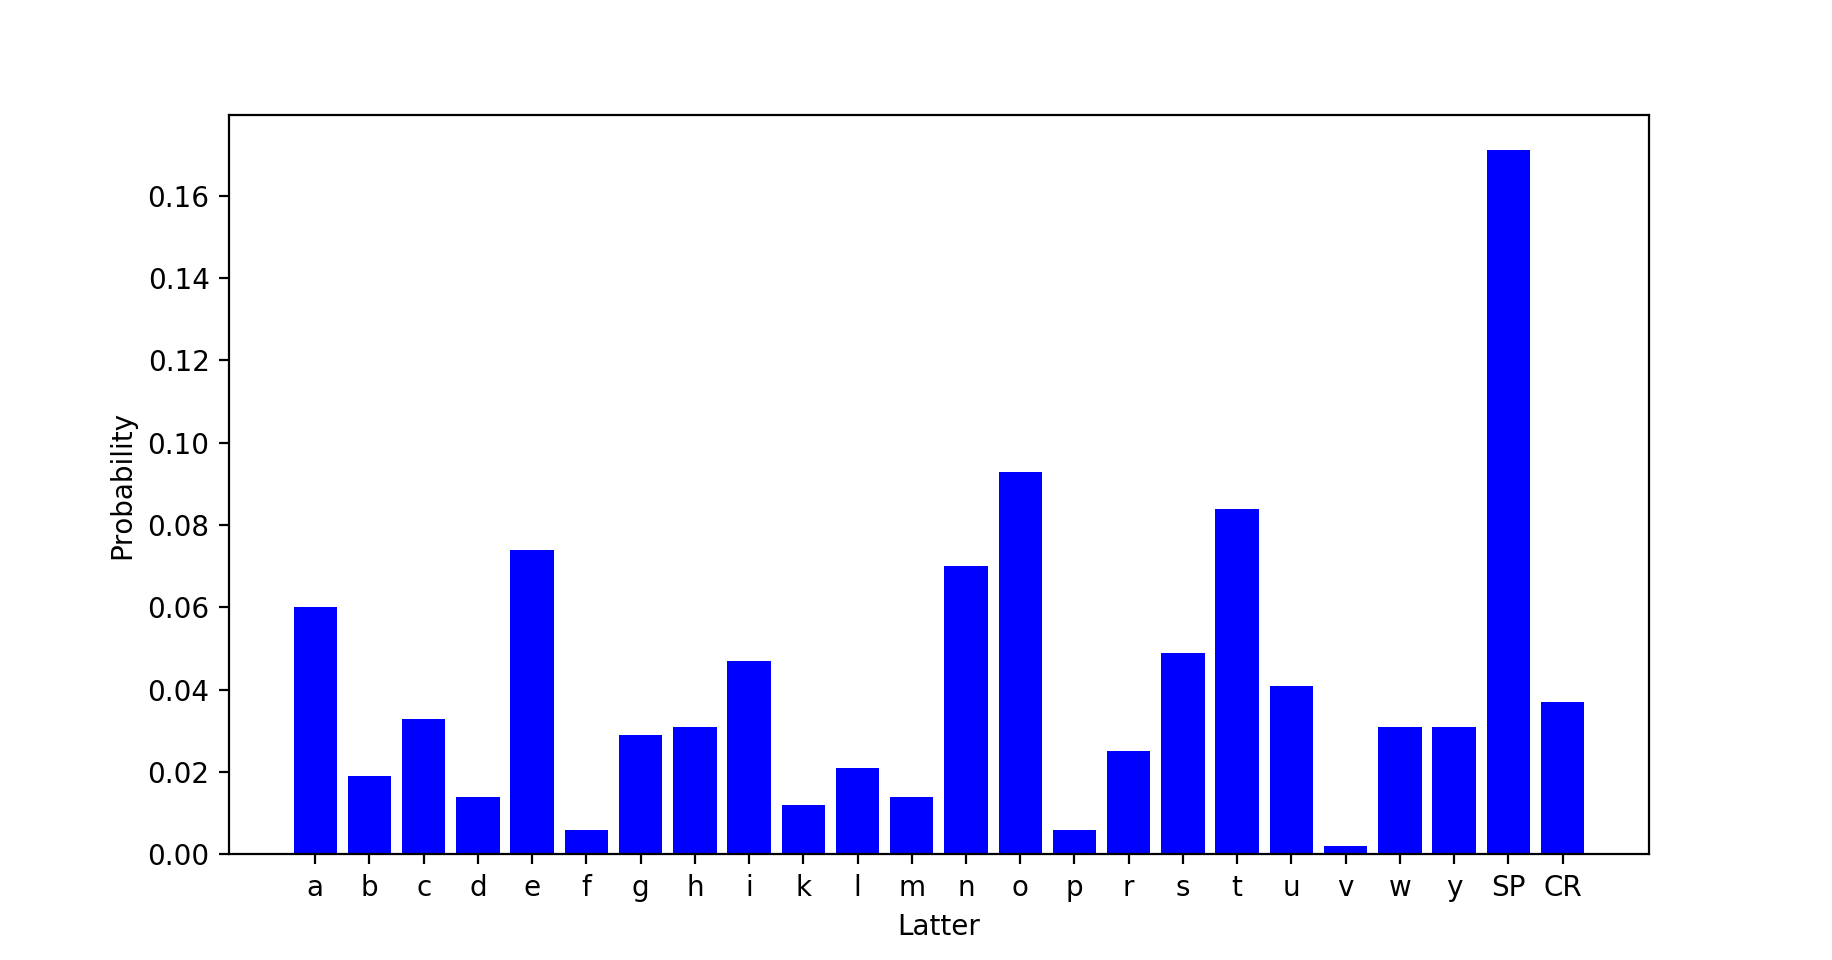
\includegraphics[width=\textwidth]{image/pmf}
	\caption{Empirical distribution for \textbf{santaclaus.txt}}
	\label{fig:empirical-distribution}
\end{figure}

\clearpage

\section*{Problem 4}
Write a program that designs a Huffman code for the given distribution in Problem 3.
\subsection*{Ans:}

\begin{figure}[h!]
	\centering
	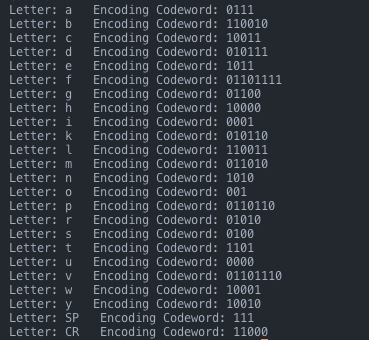
\includegraphics[width=0.8\textwidth]{image/huffman_encoding}
	\caption{Huffman encode result for \textbf{santaclaus.txt}}
	\label{fig:encode-result}
\end{figure}

\clearpage

\section*{Problem 5}
Let X be a random variable with an alphabet $H$, i.e., the 26 lower-case letters.
Use adaptive Huffman tree to find the binary code for the sequence \\ \textbf{a a b b a}.\\
You are asked to use the following 5 bits fixed-length binary code as the initial codewords for
the 26 letters. That is \\
a: 00000 \\
b: 00001 \\
\vdots \\
z: 11001 \\
\textbf{Note}: Show the Huffman tree during your coding process.
\subsection*{Ans:}

\begin{enumerate}
	\item Initial step: \\
	$Total~nodes = 2m - 1 = 26\times 2 - 1 = 51$  \\

	\hspace{3cm}

	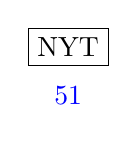
\begin{tikzpicture}
        \tikzstyle{every node}=[circle,draw]
        \node (Root)[rectangle, label={[blue]below:51}] {NYT};
	\end{tikzpicture}

	\item \textbf{a} encoded:
	\begin{multicols}{2}
        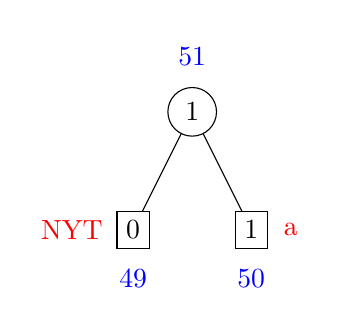
\begin{tikzpicture}
			\tikzstyle{every node}=[circle, draw]
			\node (Root)[label={[blue]above:51}] {1}
			child{
				node[rectangle, label={[red]left:NYT}, label={[blue]below:49}] {0}
			}
			child{
				node[rectangle, label={[red]right:a}, label={[blue]below:50}] {1}
			};
        \end{tikzpicture}
        
        \null \vfill
        \begin{tabular}{ cc } 
			00000 &  \\
			\textbf{a} &  \\
        \end{tabular}
		\null \vfill

	\end{multicols}
	
	\item \textbf{a a} encoded:
    \begin{multicols}{2}
        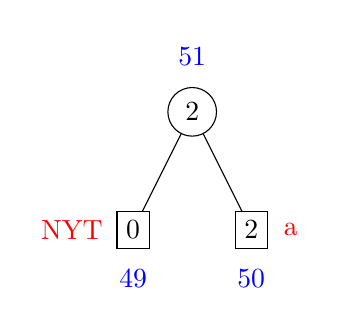
\begin{tikzpicture}
        \tikzstyle{every node}=[circle, draw]
        	\node (Root)[label={[blue]above:51}] {2}
          	child{
            	node[rectangle, label={[red]left:NYT}, label={[blue]below:49}] {0}
          	}
          	child{
            	node[rectangle, label={[red]right:a}, label={[blue]below:50}] {2}
          	};
		\end{tikzpicture} \\
		
        \null \vfill
        \begin{tabular}{ cc } 
			00000 & 1 \\
			\textbf{a} & \textbf{a} \\
        \end{tabular} \\
		\null \vfill
		
	\end{multicols}
	
	\clearpage

	\item \textbf{a a b} encoded: 
    \begin{multicols}{2}
    	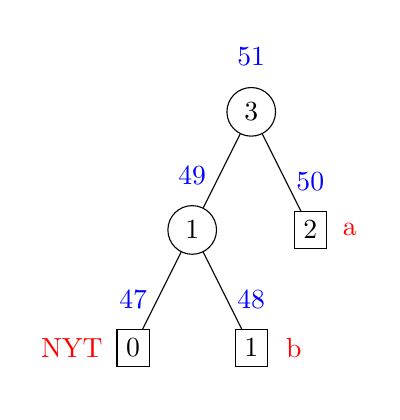
\begin{tikzpicture}
			\tikzstyle{every node}=[circle, draw]
			\node (Root)[label={[blue]above:51}] {3}
			child{
				node[label={[blue]above:49}] {1}
				child{
					node[rectangle, label={[red]left:NYT}, label={[blue]above:47}] {0}
				}
				child {
					node[rectangle, label={[red]right:b}, label={[blue]above:48}] {1}
				}
			}
			child{
				node[rectangle, label={[red]right:a}, label={[blue]above:50}] {2}
			};
		\end{tikzpicture} \\
		
        \null \vfill
        \begin{tabular}{ cccc } 
			00000 & 1 & 0 & 00001\\
			\textbf{a} & \textbf{a} & \textbf{NYT} & \textbf{b}\\
        \end{tabular} \\
		\null \vfill
		  
	\end{multicols}
	
	\item \textbf{a a b b} encoded: 
	\begin{multicols}{2}
		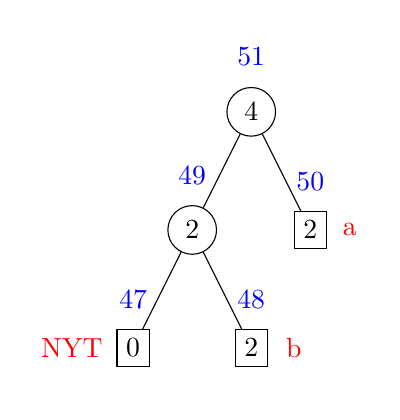
\begin{tikzpicture}
		\tikzstyle{every node}=[circle, draw]
		\node (Root)[label={[blue]above:51}] {4}
			child{
				node[label={[blue]above:49}] {2}
				child{
					node[rectangle, label={[red]left:NYT}, label={[blue]above:47}] {0}
				}
				child {
					node[rectangle, label={[red]right:b}, label={[blue]above:48}] {2}
				}
			}
			child{
				node[rectangle, label={[red]right:a}, label={[blue]above:50}] {2}
			};
		\end{tikzpicture} \\

		\null \vfill
		\begin{tabular}{ ccccc } 
			00000 & 1 & 0 & 00001 & 01\\
			\textbf{a} & \textbf{a} & \textbf{NYT} & \textbf{b} & \textbf{b}\\
		\end{tabular} \\
		\null \vfill

	\end{multicols}
	
	\item \textbf{a a b b a} encoded:
    \begin{multicols}{2}
		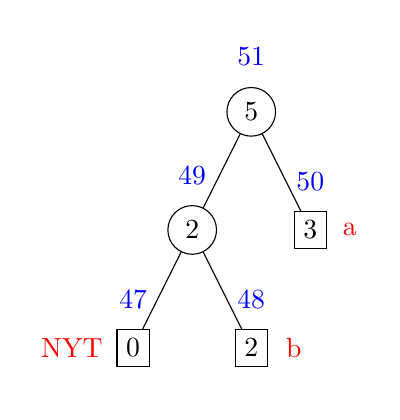
\begin{tikzpicture}
		\tikzstyle{every node}=[circle, draw]
		\node (Root)[label={[blue]above:51}] {5}
			child{
				node[label={[blue]above:49}] {2}
				child{
					node[rectangle, label={[red]left:NYT}, label={[blue]above:47}] {0}
				}
				child {
					node[rectangle, label={[red]right:b}, label={[blue]above:48}] {2}
				}
			}
			child{
				node[rectangle, label={[red]right:a}, label={[blue]above:50}] {3}
			};
		\end{tikzpicture} \\

		\null \vfill
		\begin{tabular}{ cccccc } 
			00000 & 1 & 0 & 00001 & 01 & 1\\
			\textbf{a} & \textbf{a} & \textbf{NYT} & \textbf{b} & \textbf{b} & \textbf{a}\\
		\end{tabular} \\
		\null \vfill

    \end{multicols}
	
\end{enumerate}

\clearpage

\section*{Problem 6}
\begin{enumerate}[label=(\alph*)]
	\item Find the Golomb code of n=21 when m=4.
	\subsection*{Ans:}
	\begin{align*}
		&2^{\ceil*{\log_2^{m}}}-m=2^{2}-4 = 0 \\
      	&encoding~21 = 21 \div 4 = 5 \dots 1 = 111110~01 
	\end{align*}

	\item Find the Golomb code of n=14 when m=4.
	\subsection*{Ans:}
	\begin{align*}
		&2^{\ceil*{\log_2^{m}}}-m=2^{2}-4 = 0 \\
		&encoding~14 = 14 \div 4 = 3 \dots 2 = 1110~10 
	\end{align*}

	\item Find the Golomb code of n=21 when m=5.
	\subsection*{Ans:}
	\begin{align*}
		&2^{\ceil*{\log_2^{m}}}-m=2^{3}-5 = 3 \\
		&encoding~21 = 21 \div 5 = 2 \dots 1 = 110~01 
	\end{align*}

	\item Find the Golomb code of n=14 when m=5.
  	\subsection*{Ans:}
    \begin{align*}
		&2^{\ceil*{\log_2^{m}}}-m=2^{3}-5 = 3 \\
		&encoding~14 = 14 \div 5 = 2 \dots 4 = 110~111 
	\end{align*}
	
	\item A two-integer sequence is encoded by Golomb code with m=4 to get the bitstream
  	11101111000. What’s the decoded two-integer sequence?
  	\subsection*{Ans:}
    \begin{align*}
		&2^{\ceil*{\log_2^{m}}}-m=2^{2}-4 = 0 \\
		&\begin{tabular}{ cccc } 
			\underline{1110} & \underline{11} & \underline{110} & \underline{00} \\
			3                & 3              & 2               & 0 \\
		\multicolumn{2}{c}{15} & \multicolumn{2}{c}{8} \\
		\multicolumn{4}{c}{sequence: 15, 8} 
		\end{tabular} \\
	\end{align*}
	
	\clearpage

	\item A two-integer sequence is encoded by Golomb code with m=5 to get the bitstream
	11101111000 (the same bitstream as that in (e)). What’s the decoded two-integer sequence?\\
	\textbf{Hint}: The unary code for a positive integer $q$ is simply $q$ 1s followed by a $0$.
	\subsection*{Ans:}
	\begin{align*}
		&2^{\ceil*{\log_2^{m}}}-m=2^{3}-5 = 3 \\
		&\begin{tabular}{ cccc } 
		\underline{1110} & \underline{111} & \underline{10} & \underline{00} \\
		3                & 7-3 = 4         & 1              & 0 \\
		\multicolumn{2}{c}{19} & \multicolumn{2}{c}{5} \\
		\multicolumn{4}{c}{sequence: 19, 5} 
		\end{tabular} \\
	\end{align*}


\end{enumerate}

\clearpage

\subsection*{Source code for Problem 3 \& 4}
\textit{huffman.py}
\lstinputlisting[language=Python]{huffman.py}
\textit{main.py}
\lstinputlisting[language=Python]{main.py}

\end{document}